\documentclass[12pt,titlepage]{scrartcl}
\usepackage[ngerman]{babel}
\usepackage[utf8]{inputenc}
\usepackage[a4paper,lmargin={2.5cm},rmargin={2.5cm},tmargin={2.5cm},bmargin={2.5cm}]{geometry}
\usepackage{graphicx}
\usepackage[T1]{fontenc}
\usepackage[headsepline,footsepline, singlespacing=true]{scrlayer-scrpage}
\usepackage{mwe}
\usepackage{acronym}
\usepackage{blindtext}
\usepackage[hidelinks]{hyperref}
\usepackage{csquotes}
\usepackage{setspace}
\usepackage[ngerman]{cleveref}

\usepackage[
  backend=biber,
  style=ext-authoryear,
  maxcitenames=2, maxbibnames=999,
  giveninits=true,
  uniquename=init, uniquelist=false,
  articlein=false, innamebeforetitle=true,
  punctfont=true, dashed=false,
]{biblatex}

% !TEX root = twe2.tex

%Zitierstil latex beibringen
\DefineBibliographyStrings{ngerman}{
	andothers = {{et\,al\adddot}}
}

\newcommand{\fontForTheSeminar}{ppl}
\renewcommand*{\mkbibnamefamily}{\expandafter\MakeUppercase\expandafter}
\AtBeginBibliography{%
  \renewcommand*{\mkbibnamefamily}[1]{#1}}

\DeclareNameFormat{labelname}{%
  \ifnum\value{uniquename}=0\relax
    \usebibmacro{name:family}
      {\namepartfamily}
      {\namepartgiven}
      {\namepartprefix}
      {\namepartsuffix}%
  \else
    \usebibmacro{name:family-given}
      {\namepartfamily}
      {\namepartgiveni}
      {\namepartprefix}
      {\namepartsuffixi}%
  \fi
  \usebibmacro{name:andothers}}

\DeclareNameAlias{default}{family-given}
\DeclareNameAlias{sortname}{default}

\DeclareDelimAlias*[bib]{finalnamedelim}{multinamedelim}
\setlength{\bibhang}{0pt}

\DeclareNameWrapperFormat{sortname}{\mkbibbold{#1}}
\DeclareFieldFormat{biblabeldate}{\mkbibbold{\mkbibparens{#1}}}
\DeclareFieldFormat{journaltitle}{#1\isdot}
\DeclareFieldFormat*{title}{#1}

\DeclareDelimFormat[bib]{nametitledelim}{\addcolon\space}

\renewcommand*{\volnumdelim}{\addcomma\space}

\DeclareFieldFormat{pages}{#1}

\renewcommand*{\bibpagespunct}{\addcolon\ifentrytype{article}{}{\space}}

\DeclareDelimFormat{postnotedelim}{\addcolon}
\DeclareFieldFormat{postnote}{\mknormrange{#1}}
\setlength\bibitemsep{6pt}

\renewcommand*{\bibfont}{\normalsize}

%Schriftwahl
\newcommand{\changefont}[3]{\fontfamily{#1} \fontseries{#2} \fontshape{#3} \selectfont}


\addbibresource{bibtex/bib.bib}

\setlength{\parindent}{0pt}
\RedeclareSectionCommand[%
	beforeskip=32pt,
	afterskip=6pt,
	runin=false]{section}

\RedeclareSectionCommand[%
	beforeskip=12pt,
	afterskip=6pt,
	runin=false]{subsection}

\RedeclareSectionCommand[%
	beforeskip=12pt,
	afterskip=6pt,
	runin=false]{subsubsection}

\pagestyle{scrheadings}
\changefont{\fontForTheSeminar}{m}{n}
\linespread{1.3}
\flushbottom


\begin{document}
\changefont{\fontForTheSeminar}{m}{n}

% !TEX root = twe2.tex

\begin{titlepage}
\changefont{\fontForTheSeminar}{m}{n}
\centering

\begingroup
    \Large{Fachhochschule Kiel}
    \par
\endgroup

\begingroup
    \large{Hochschule für Angewandte Wissenschaften \\
        Fachbereich Agrarwirtschaft \\
        Osterrönfeld}
    \par
\endgroup


\vspace{3cm}


\begingroup
    \Large
    \bfseries{Seminar II}
    \par
\endgroup

\vspace{0.1cm}

im Studienfach Landwirtschaft

\vspace{2cm}

\hrulefill

\vspace{0.5cm}
\begingroup
    \LARGE
    \bfseries{Leguminosen für zusätzliches Protein aus dem Grünland}
    \par
\endgroup
\vspace{0.5cm}
\hrulefill
\vspace{2cm}

vorgelegt von:

\begingroup
    \large{Tibor Weiß}
    \par
\endgroup

\vspace{1.5cm}

betreut von:

\begingroup
    \large{Prof. Dr. Rainer Wulfes \\
        Prof. Dr. John B. Goodenough}
    \par
\endgroup

\vspace{2cm}

Osterrönfeld, im Oktober 2020

\end{titlepage}


%einige letzte Befehle für das Layout
\setlength{\parskip}{9pt} %Abstand nach Absatz
\newpage %neue Seite nach dem DEckblatt
\clearpairofpagestyles %alle Layouteinstellungen vom Deckblatt löschen
\changefont{\fontForTheSeminar}{m}{n} %Schrift aktualisieren
\ohead{\headmark} %Kopfzeile
\ofoot{\pagemark} %Fußzeile
\automark{section} %aktuelle Section wird in der Kopfzeile angezeigt
\renewcommand*{\sectionmarkformat}{} %Darstellung Section in der Kopfzeile angepasst
\setcounter{page}{2} %Seitenzähler auf 2 Stellen


%Inhaltsverzeichnis
\tableofcontents


%Tabellen- und Abbildungsverzeichnis
%\listoftables
%\listoffigures
%Anhangsverzeichnis TODO

%Abkürzungsverzeichnis - Abkürzungen eintragen
\section*{Abkürzungsverzeichnis}
\addcontentsline{toc}{section}{Abkürzungsverzeichnis}
\begin{acronym}[AGGF] %die längste Abkürzung in die eckigen Klammern schreiben für tabellarische Darstellung
	\acro{AGGF}{Arbeitsgemeinschaft Grünland und Feldfutterbau}
	\acro{NEL}{Netto-Energie-Laktation}
	\acro{TM}{Trockenmasse}
	\acro{XP}{Rohprotein}
\end{acronym}
\newpage

% !TEX root = twe2.tex


\section{Einleitung}
\label{sec:Einleitung}

Unter den strengeren Auflagen bzgl. der Düngung von landwirtschaftlich genutzten Flächen sowie einer Optimierung der Nutzung des Grünlandes in der Milchviehhaltung steigen die Anforderungen an das Grünland.
Insbesondere die \ac{NEL} Erträge stehen dabei im Fokus.
Die \ac{AGGF} hat sich im Rahmen Ihrer 63. Jahrestagung unter dem Motto "Grünland 2050" getroffen.
\textcite[33-36]{weggler2050leguminosen} haben sich mit der Möglichkeit der Steigerung des Leguminosen-Anteils und der Reduzierung der N-Düngung beschäftigt.

Da Leguminosen Stickstoff aus der Luft binden können sind diese nicht auf eine ausreichende N-Düngung angewiesen und sind gegenüber Gras bei intensiver N-Düngung nicht konkurrenzfähig.
Allerdings haben Leguminosen aufgrund ihrerer Stickstofffixierung sehr hohe Proteingehalte ohne dabei auf eine intensive N-Düngung angewiesen zu sein.
Dies wirft die Frage auf, ob ein bestimmter Leguminosenanteil in der Gräsermischung bei gleichzeitiger Reduktion der N-Düngung in der Lage ist höhere \ac{NEL}-Erträge zu liefern.
Damit die Grasnarbe gegenüber unerwünschten Pflanzen einen ausreichend konkurrenzfähig ist, ist eine ausreichende Stickstoffversorgung der Gräser sehr wichtig.
Somit ist ein Ausgleich der Interessen der Gräser und Leguminosen notwendig um die \ac{NEL}-Erträge zu optimieren.
Daher liegt hier ein klasisches mehrdimensionales Optimierungsproblem vor.

Die Einflüsse auf die Umwelt über eine geringere N-Düngung sind politisch gewollt.
Dies wird nicht untersucht und somit richtet sich der Artikel eindeutig an die Landwirtschaft und nicht an die Politik.



% !TEX root = twe2.tex

\section{Literatur}
\label{sec:Literatur}

Aufgrund der preiswerten Versorgung von Proteinen über importiertes Soja ist die Steigerung der \ac{NEL}-Erträge zu Lasten der \ac{TM}-Erträge bisher relativ uninteressant gewesen.
Inzwischen verlangen aber immer mehr Verbraucher Produkte welche unter Gesichtspunkten des Umweltschutzes und Ressourcenschonung produziert wurden.
Dadurch ist der Einsatz von importierten Soja für einige Betriebe nicht mehr möglich bzw. erschwert die Vermarktung der Milch und diese Milcherzeuger müssen daher andere Proteinquellen erschließen.

\subsection{Einfluss auf TM-Erträge}
\label{subsec:TM}

Die Grasbestände sind insbesondere auf einen hohen \ac{TM}-Ertag ausgelegt.
Dieser wird über sehr ertragsreiche, aber auch auf N-Düngung angewiesenen Arten und Sorten erreicht.
Allerdings hat sich bereits gezeigt, dass eine Artenreiche Gräsermischung, insbesondere mit Leguminosen, höhere Erträge liefern können als Reinsaaten der ertragreichsten Art \parencite{nyfeler2009strong}.\todo{Seitenzahl einfügen!}
Leguminosen reduzierne die N\textsubscript{2}-Fixierung bei N-Düngung \parencite{ledgard2001nitrogen}\todo{Seitenzahl einfügen}, weswegen die N-Düngung zumindestens reduziert werden muss \parencite[34]{weggler2050leguminosen}.

Bei einer Reduzierung der N-Düngung um die Leguminosen in den Bestand zu integrieren ist daher zu befürchten, dass die \ac{TM}-Erträge absinken werden.
Dies ist zu vermeiden, da viele Betriebe darauf angewiesen sind, mit den vorhanden Flächen ausreichend Futter für Ihre Tiere zu produzieren.
Nach \textcite[11]{engel2013protein} sind die Verluste an \ac{TM} Ertrag bei einer Reduzierung der N-Düngung von 240 kg N ha\textsuperscript{-1}a\textsuperscript{-1} ohne Leguminosen auf 80 kg N ha\textsuperscript{-1}a\textsuperscript{-1} mit Weißklee bei etwa 20\%.

Allerdings ist auch zu erwähnen, dass eine Düngung von 240 kg N ha\textsuperscript{-1}a\textsuperscript{-1} eventuell im Zuge der Agrarpolitik von der \ac{EU} verboten oder eingeschränkt wird.
Daher scheint der Vergleich von 160 kg N ha\textsuperscript{-1}a\textsuperscript{-1} ohen Leguminosen mit 80 kg N ha\textsuperscript{-1}a\textsuperscript{-1} unter langfristigen Gesichtspunkten angebrachter.
In diesem Fall reduziert sich der \ac{TM} Ertrag nach \textcite[11]{engel2013protein} um etwa 2,5\%.
Leider sind keine Konfidenzintervalle angegeben, sodass eine Aussage über die statistische Signifikanz hier leider nicht möglich ist.

Nach \textcite[35-36]{weggler2050leguminosen} sind die \ac{NEL} Erträge je Hektar bei Rotklee größer als bei Weißklee, allerdings sinkt der Gehalt an \ac{XP}.
Dies bedeutet, dass mit einer Rotkleenachsaat nicht nur der \ac{NEL} Ertrag gesteigert werden kann, sondern auch der \ac{TM} Ertrag.
Allerdings geht dies zu Lasten des \ac{XP} Gehalts in dem Aufwuchs.
Da die Futteraufnahme der Tiere begrenzt ist, ist mit einem Rückgang der Milchleistung aus dem Grundfutter zu rechnen.

\subsection{Einfluss auf Proteingehalt}
\label{subsec:Protein}

Auch wenn Leguminosen generell die Möglichkeit haben höhere \ac{XP}gehalte zu generieren, stellt sich die Frage ob eine Nachsaat von Leguminosen ausreicht um die \ac{XP}gehalte bei einer Reduizierung der N-Düngung konstant zu halten.
Nach \textcite[35]{weggler2050leguminosen} ist es möglich die \ac{XP}gehalte zu steigern.

\subsection{Mineralische N-Düngung}
\label{subsec:Lit:N-Düngung}

Da in der Milchviehhaltung generell eine ausreichende Menge Gülle anfällt, ist davon auszugehen, dass die Grünlandflächen den größten Teil ihrer Düngung über die Gülle bekommen.
Insbesondere die Stickstoffversorgung ist derzeit eher unproblematisch aufgrund der über das Kraftfutter in den Kreislauf eingebrachten Eiweiße.
Daher wird derzeit nur ein kleiner Teil der Stickstoffversorgung des Grünlandes über mineralischen Dünger abgebildet.
Dies ist problematisch, da die organische Düngung nur mit relativ hohem Aufwand reduziert werden kann.
Die Gülle muss an andere Betriebe abgegeben werden und mineralischer Phosphor- und insbesondere Kalidünger muss den Bedarf der Pflanzen decken.
Bei einer Reduzierung der Eiweißkonzentration im Kraftfutter ist davon auszugehen, dass der Stickstoffgehalt der Gülle auch absinkt.

\subsection{Ernteverluste}
\label{subsec:Lit:Ernte}

Nachdem die \ac{XP} erfolgreich auf dem Feld produziert wurden, müssen diese konserviert werden.
Jeder Verlust von \ac{XP} in der Ernte muss entweder über den Zukauf oder über geringere Milchleistung bezahlt werden.
Über lagen Feldliegezeiten, hohe Bröckelverluste und ähnliches steigen die \ac{XP}-Verluste.

\subsubsection{Silage}
\label{subsub:Silage}
Bei der Silierung treten Silierungsverluste auf, desweiteren können bei nicht ausreichender Verdichtung, kein Luftabschluss oä Fehlgärungen auftreten.
Die Ernteverluste betragen etwa 22\% \parencite[30]{fritz2018wirtschaftliche}.


\subsubsection{Grascobs}
\label{subsub:Peletts}
Sehr aufwendig, geringe Verluste \parencite[12f]{engel2013protein}

\subsubsection{Heu}
\label{subsub:Heu}
Lange Feldliegezeit oder teure Heutrocknung, Ernteverluste \ac{NEL} zwischen 33\% und 21\% \parencite[30]{fritz2018wirtschaftliche}.



% !TEX root = twe2.tex

\section{Diskussion}
\label{sec:Disukussion}
\textcite[33-36]{weggler2050leguminosen} hat Möglichkeiten zur Steigerung der \ac{NEL} Erträge im Grünland aufgezeigt, allerdings ist zu beachten, dass aktuelle Verfahren der Futterkonxerierung zu hohen Verlusten führen, siehe \cref{subsec:Lit:Ernte}. \todo{ausformulieren}
Mit zukünftigen Ernte- und Konservierungsverfahren werden Landwirte hoffentlich Möglichkeiten haben die Verluste zu reduzieren.

\subsection{Literaturkritik}
\label{sub:kritik}

\begin{figure}
	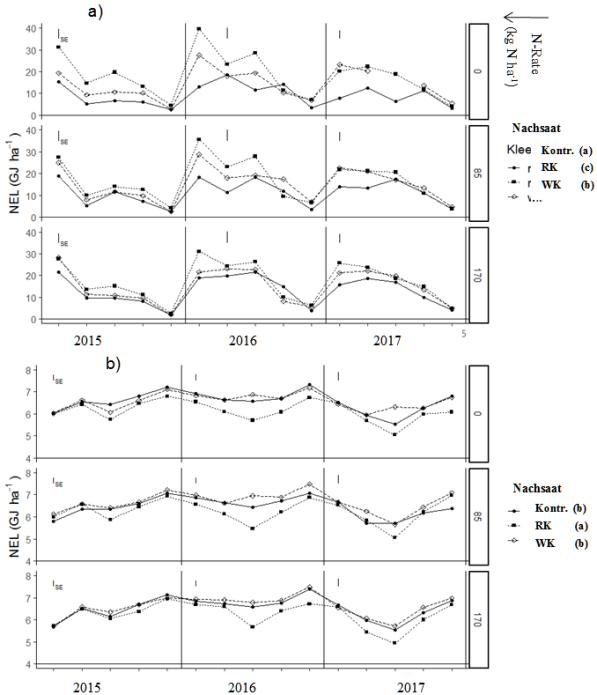
\includegraphics[scale=0.5]{images/wegglerAbb1}
	\caption[(a) \acs{NEL} Ertrag und (b) \acs{NEL} Konzentration in Abhängigkeit von der N-Düngung und Leguminosen Nachsaat über 3 Jahre]{(a) \ac{NEL} Ertrag und (b) \ac{NEL} Konzentration in Abhängigkeit von der N-Düngung und Leguminosen Nachsaat über 3 Jahre \parencite[35]{weggler2050leguminosen}}
	\label{fig:wegglerAbb1}
\end{figure}

In dem Arikel \parencite[33-36]{weggler2050leguminosen}\todo{Seitenangabe notwendig wenn die komplette Arbeit referenziert wird?} sind einige kleinere handwerkliche Fehler enthalten.
In \textcite[35]{weggler2050leguminosen} ist die Legende sowie Achsbeschriftung, siehe \cref{fig:wegglerAbb1} nicht korrekt umgesetzt.
\todo{Numerierung ok? Verwendung Abk ok?, Breite ok? Müssen Abb. linksbündig sein?}
So wird zum Beispiel der \ac{NEL} Gehalt mit GJ ha\textsuperscript{-1} beschrfitet, statt MJ kg\textsuperscript{-1} in \ac{TM}.

Desweiteren wird die Abkürzung \ac{NEL} in der Einleitung nicht als \acl{NEL} eingeführt sondern als \textit{nutzbare Energie Laktation}.\todo{kursiv okay zum makieren von Fehlern?}
Im Kapitel Material und Methoden wird \ac{NEL} als \textit{Netto Energie Lactaion} bezeichnet.
In Abbildungsunterschriften wird widerholt \textit{nutzbare Energie Laktation} verwendet.
Normalerweise wird im landwirtschaftlichen die Abkürzung \acs{NEL} für \acl{NEL} benutzt.
Desweiteren ist \ac{NEL} eine wichtige Kenngröße in der Grundfuttermittelproduktion der Milchviehhaltung und somit der Grünlandwirtschaft.
Es findet sich kein Hinweis auf eine Meßmethode welche die \textit{nutzbare Energie Laktation} bestimmt.
Daher liegt es nahe einen Fehler in der Bezeichnung zu vermuten.

Die Darstellung der \cref{fig:wegglerAbb1} ist nicht ideal.
Die verschiedenen Messpunkte beziehen sich auf die einzelnen Aufwüchse, diese per Linie miteinander zu verbinden hilft zwar beim erkennen welcher Punkt zu welcher Datenreihe gehört.
Es gitb aber keine Datenpunkte welche zwischen den einzelnen Aufwüchsen liegt, welche man eventuell interpolieren könnte.
Wen die x-Achse die N-Düngung angeben würde und die verschiedenen Schnitte in mehrere Diagramme aufgeteil worden wären, wobei bei jedem Schnitt jeweils der Durchschnitt der 3 Jahre genommen wird, wäre die Darstellung leichter verständlich.


\subsection{Leguminosen als Proteinlieferant}
\label{sub:leguminosen}
Wie in \ref{subsec:Protein} gezeigt, können Leguminosen den \ac{XP} Ertrag vom Grünland erhöhen.
Der Versuch von \textcite[33-36]{weggler2050leguminosen} wurde allerdings nur bis zu einer Düngung von 170kg N ha\textsuperscript{-1}a\textsuperscript{-1} gesteigert.
Daher ist es schwierig, einen Vergleich zwischen einer, in Norddeutschland üblichen,\todo{Zitat einfügen} N-Düngung\todo{N in Abkürzungsliste einfügen?} von über 200kg N ha\textsuperscript{-1} sowie einer minimierten N-Düngung mit Leguminosen zu ziehen.
Eine Nachsaat mit Rotklee hatte häufig einen leicht negativen Einfluss auf den \ac{XP} Gehalt des Aufwuchs, während eine Weißlkleenachsaat tendenziell eine leichte Steigerung der \ac{XP} Gehalte zur Folge hatte.
Generell sind deutliche Steigerungen des \ac{NEL} Ertrages möglich, insbesondere bei (sehr) geringer N-Düngung, wobei insbesondere der Rotklee (siehe \ref{subsec:TM}) die \ac{TM} Erträge deutlich steigert.

Da der Rotklee zu einer signifikanten Verringerung der \ac{NEL} Konzentration des Aufwuches geführt hat, ist für Milchviehbetriebe nachteilig.
Daher scheint eine Strategie mit einer Rot- Weißklee Mischung als Nachsaat für die meisten Betriebe (zumindestens kurzfristig) sinnvoll zu sein.
Bei Betrieben, welche eine etwas geringere Viehbesatzdichte haben, kann eine Weißkleenachsaat sinnvoller sein.
In weiteren Forschungen können die betriebswirtschaftlichen Einflüsse auf die Betriebe ausgearbeitet werden um den milchviehhaltenden Betrieben eine wirtschaftliche Empfehlung geben zu können.

\subsubsection{Nährstoffkreislauf}
\label{subsub:nährstoffkreislauf}

In der Milchkuhhaltung besteht ein Nährstoffkreislauf.
Über den Verkauf von Milch verlassen Nährstoffe, insbesondere N in Form des Milcheiweißes, den Betrieb.
Falls der Betrieb den Wirtschaftsdünger abgibt, bzw. abgeben muss, verlassen darüber weitere Nährstoffe den Betrieb, unter anderem N.
Nährstoffeinträge sind insbesondere über den Zukauf von Kraftfutter sowie, in eher geringen Mengen, der Einsatz von mineralischen Düngemitteln.
Der Einsatz von Kraftfuttern ist für eine Milchkuh zur Steigerung der Milchleistung sehr sinnvoll.
Eine Redufzierung des Kraftuffters ist, in den meisten Fällen, unwirtschaftlich.

Bei einer Reduzierung der N-Düngung auf den betriebseigenen Grünlandflächen ist, in den meisten Fällen, nicht mehr genügend Fläche vorhanden, um die eigenen Wirtschaftsdünger innerhalb des Betriebes zu verwerten.
Aufgrund der hohen Transportkosten ist eine Vewertung im nahem Umkreis anzustreben.
Insbesondere in Regionen mit einer hohen Besatzdichte an Milchkühen entsteht somit ein Überschuss an Wirtschaftsdüngern welcher exportiert werden muss.
Dies ist für die dort angesiedelten Betriebe eine große wirtschaftliche Herausforderung.
Nicht nur aufgrund der Transportkosten, welche in der Regel der abgebende Betrieb tragen muss, sondern auch, weil die anderen abgegeben Nährstoffe wieder zugekauft werden müssen.

\subsubsection{Leguminosen als alternative zu Kraftfutter}
\label{subsub:alternative}
Bei einem Einsatz von Leguminosen in der Grundfuttergewinnung ist eine Steigerung der \ac{NEL}-Eträge möglich.
Eine Reduzierung der Kraftfuttergabe ist, zumindestens für die meisten Betriebe, nicht wirtschaftlich.
Über das Kraftfutter wird kein Raufutter substituiert, daher ist der Einsatz von Kraftuffter unabhängig von der Qualität des Raufutters zu bewerten.

Falls Kraftfutter deutlich teuerer werden sollte, kann es sein, dass der Einsatz nicht mehr wirtschaftlich sinnvoll ist.
Die \ac{EU} könnte z.B. Importzölle auf Soja erheben, generell den Kraftfuttereinsatz einschränken oder ähnliche Einschränkungen beschließen.
Da insbesondere Soja aus Südamerika gesellschaftlich in der Kritik steht, kann es passieren, dass die \ac{EU} sich zum handeln gezwungen sieht.

Für den Fall dass der Eintrag von N über das Kraftfutter in den Nährstoffkreislauf deutlich reduziert wird, ändern sich die Vorraussetzungen.
Da der Verlust über den Verkauf von Milch bestehen bleibt, müssen neue Quellen erschlossen werden.
Eine Möglichkeit ist der Einsatz von mineralischen N-Düngemitteln, eine andere Möglichkeit wäre der Einsatz von Leguminosen.
In diesem Fall, je nach Entwicklung der Preise und bessierend auf den Ergebnissen von \textcite[33-36]{weggler2050leguminosen}, könnte eine Leguminosennachsaat kostengünstgier sein.


\subsection{Effizienz der Konservierung}
\label{sub:konservierung}
\ac{NEL} Verluste während der Ernte, Konservierung oder Lagerung sind besonders kritisch zu betrachten.
Nachdem der Landwirt aufwändig hochwertiges Futter erzeugt hat, verliert dieses etwa 20\% des \ac{NEL} Ertrags.
Diese Verluste sind aus betriebswirtschaftlicher Sicht langfristig nicht zu rechtfertigen.
Die Reduzierung dieser Verluste wird immer wichtiger, da vermutlich größere Anteile der \ac{NEL} über das Grundfutter abgedeckt werden muss.
Eine Verbesserung der Ernteverfahren bzw. Konservierungsmethoden ist daher dringend geboten.
Es bleibt somit zu hoffen dass die Forschung neue wirtschaftliche Verfahren entwickelt welche eine wirtschaftliche Nutzung des kompletten \ac{NEL} Ertrags von landwirtschaftlichen Flächen erlaubt.

\subsection{Fazit}
\label{subsec:fazit}
Leguminosen sind eine sinnvolle Variante um die \ac{NEL} Erträge des Grünlandes zu steigern.
Neben der Steigerung der Erträge wäre eine effizientere Verwertung dieser wünschenswert.


% !TEX root = twe2.tex

\section{Zusammenfassung}
\label{sec:Zusammenfassung}

Die Steigerung der \ac{NEL} Erträge von den Grünlandflächen ist für Milchvieh haltende Betriebe eine wichtige Aufgabe.
Eine Nachsaat mit Weiß- und Rotklee kann \ac{NEL} Erträge auch bei minimaler N Düngung etwas über dem Niveau einer Düngung mit 170 kg N ha\textsuperscript{-1}a\textsuperscript{-1} halten.
Dies ist unter dem Gesichtspunkten der höheren Auflagne an die N-Düngung eine wichtige Erkenntnis.
So können Milchviehbetriebe auf dem Grünland den Einsatz von N-Düngemittel potentiel deutlich reduzieren.
Allerdings erfolgt ein großteil der N-Düngung bereits über den Wirtschaftsdünger der Betriebe.
Eine Reduzierung der N-Düngung würde diese Betriebe dazu zwingen, einen Teil des Wirtschaftsdünger zu exportieren.
Bei dem momentanen Einsatz von Düngemittel scheint eine Steigerung von ca. 10\% möglich zu sein.
Das Potential von einer Steigerung von 25\% bei einer besseren Futterkonservierung ist nicht zu vernachlässigen.


%Literaturverzeichnis
\begin{singlespace} %einfacher Zeilenabstand im Literaturverzeichnis
\begin{flushleft} %linksbündig
\addcontentsline{toc}{section}{Literaturverzeichnis}
\printbibliography[title=Literaturverzeichnis]
\end{flushleft}
\end{singlespace}

%Anhang
\end{document}
